% Standalone overview of fastrho tokenization and model architecture.
% Regenerate through the repository-level reproduce workflow.
\documentclass[border=4pt]{standalone}
\usepackage{tikz}
\usepackage{amsmath,amssymb}
\usepackage{helvet}
\renewcommand{\familydefault}{\sfdefault}
\usetikzlibrary{arrows.meta,backgrounds,calc,fit,positioning}

\definecolor{frblue}{HTML}{2737E7}
\definecolor{frink}{HTML}{151515}
\definecolor{frgrey}{HTML}{777777}
\definecolor{frrule}{HTML}{CFCFCF}

\begin{document}
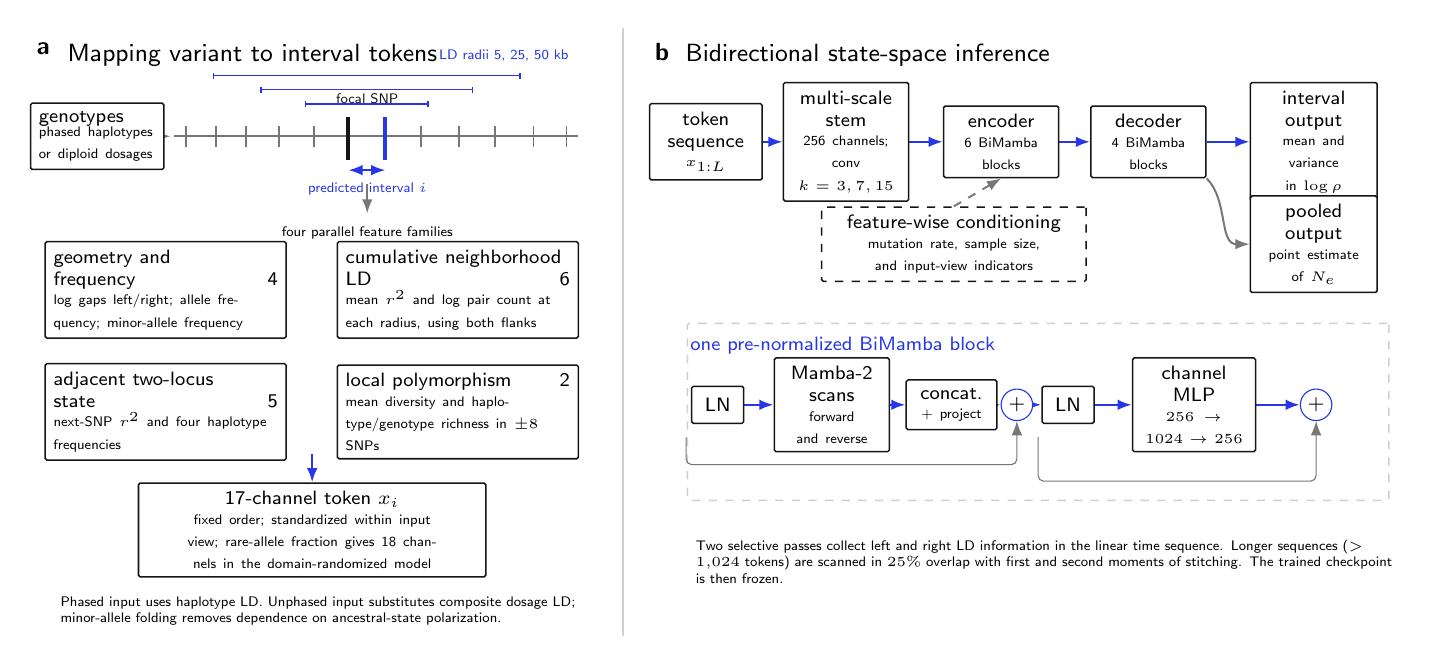
\begin{tikzpicture}[
  x=1cm,y=1cm,
  font=\sffamily\scriptsize,
  >={Latex[length=1.8mm]},
  flow/.style={->,draw=frgrey,line width=0.72pt},
  blueflow/.style={->,draw=frblue,line width=0.88pt},
  card/.style={draw=frink,rounded corners=0.6pt,fill=white,line width=0.55pt,
               inner sep=3pt,align=left},
  bluecard/.style={card},
  greencard/.style={card},
  purplecard/.style={card},
  orangecard/.style={card,dashed},
  smallnote/.style={font=\sffamily\tiny,text=black,align=left},
  paneltitle/.style={font=\sffamily\small,anchor=north west},
]
\pgfdeclarelayer{connections}
\pgfsetlayers{background,connections,main}

% A single structural rule replaces decorative panel fields.
\begin{pgfonlayer}{background}
\draw[frrule,line width=0.55pt] (7.75,0.20) -- (7.75,7.92);
\end{pgfonlayer}

% ------------------------------------------------------------------ panel a
\node[font=\sffamily\small\bfseries,anchor=north west] at (0.18,7.86) {a};
\node[paneltitle] at (0.57,7.84) {Mapping variant to interval tokens};

\node[card,text width=1.48cm,minimum height=0.82cm] (input) at (1.07,6.55)
  {genotypes\\[-1pt]\tiny phased haplotypes\\or diploid dosages};

% A focal SNP predicts the interval immediately to its right.
\draw[frgrey,line width=0.75pt] (2.05,6.55) -- (7.18,6.55);
\foreach \x in {2.20,2.58,2.96,3.38,3.82,4.26,4.73,5.18,5.66,6.12,6.61,7.03}
  \draw[frgrey,line width=0.65pt] (\x,6.42) -- (\x,6.68);
\draw[frink,line width=1.45pt] (4.26,6.25) -- (4.26,6.79);
\draw[frblue,line width=1.45pt] (4.73,6.25) -- (4.73,6.79);
\draw[<->,frblue,line width=0.78pt] (4.26,6.12) -- (4.73,6.12);
\node[smallnote,text=frblue,anchor=north] at (4.50,6.08) {predicted interval $i$};
\draw[frblue,line width=0.45pt] (3.72,6.96) -- (5.27,6.96);
\draw[frblue,line width=0.45pt] (3.15,7.14) -- (5.84,7.14);
\draw[frblue,line width=0.45pt] (2.55,7.32) -- (6.44,7.32);
\foreach \x/\y in {3.72/6.96,5.27/6.96,3.15/7.14,5.84/7.14,2.55/7.32,6.44/7.32}
  \draw[frblue,line width=0.45pt] (\x,{\y-0.04}) -- (\x,{\y+0.04});
\node[smallnote,text=frblue,anchor=south east] at (7.18,7.38)
  {LD radii 5, 25, 50 kb};
\node[smallnote,text=frink,anchor=south] at (4.50,6.84) {focal SNP};
\begin{pgfonlayer}{connections}
\draw[flow] (input.east) -- (2.00,6.55);
\end{pgfonlayer}

% The exact 17 channels are grouped into four readable families.
\node[bluecard,text width=2.85cm,minimum height=1.02cm] (geom) at (1.94,4.60)
  {geometry and\\frequency \hfill 4\\[-1pt]
   \tiny log gaps left/right; allele frequency; minor-allele frequency};
\node[bluecard,text width=2.85cm,minimum height=1.02cm] (ld) at (5.65,4.60)
  {cumulative neighborhood\\LD \hfill 6\\[-1pt]
   \tiny mean $r^2$ and log pair count at each radius, using both flanks};
\node[greencard,text width=2.85cm,minimum height=1.02cm] (pair) at (1.94,3.05)
  {adjacent two-locus\\state \hfill 5\\[-1pt]
   \tiny next-SNP $r^2$ and four haplotype frequencies};
\node[purplecard,text width=2.85cm,minimum height=1.02cm] (local) at (5.65,3.05)
  {local polymorphism \hfill 2\\[-1pt]
   \tiny mean diversity and haplotype/genotype richness in $\pm8$ SNPs};

\begin{pgfonlayer}{connections}
\draw[flow] (4.50,5.94) -- (4.50,5.57);
\end{pgfonlayer}
\node[smallnote,anchor=north] at (4.50,5.53) {four parallel feature families};

\node[bluecard,text width=4.20cm,minimum height=0.74cm,align=center] (token) at (3.80,1.55)
  {17-channel token $x_i$\\[-1pt]
   \tiny fixed order; standardized within input view; rare-allele fraction gives 18 channels in the domain-randomized model};
\begin{pgfonlayer}{connections}
\draw[blueflow] (3.80,2.52) -- (token.north);
\end{pgfonlayer}
\node[smallnote,text width=6.75cm,anchor=north west] at (0.48,0.83)
  {Phased input uses haplotype LD. Unphased input substitutes composite dosage LD;
   minor-allele folding removes dependence on ancestral-state polarization.};

% ------------------------------------------------------------------ panel b
\node[font=\sffamily\small\bfseries,anchor=north west] at (8.03,7.86) {b};
\node[paneltitle] at (8.42,7.84) {Bidirectional state-space inference};

% Main data path: keep only the quantities needed to understand the model.
\node[bluecard,text width=1.22cm,minimum height=0.78cm,align=center] (matrix) at (8.80,6.48)
  {token sequence\\[-1pt]\tiny $x_{1:L}$};
\node[bluecard,text width=1.38cm,minimum height=0.78cm,align=center] (stem) at (10.58,6.48)
  {multi-scale stem\\[-1pt]\tiny 256 channels; conv $k=3,7,15$};
\node[bluecard,text width=1.25cm,minimum height=0.78cm,align=center] (enc) at (12.55,6.48)
  {encoder\\[-1pt]\tiny 6 BiMamba blocks};
\node[bluecard,text width=1.25cm,minimum height=0.78cm,align=center] (dec) at (14.42,6.48)
  {decoder\\[-1pt]\tiny 4 BiMamba blocks};
\node[greencard,text width=1.40cm,minimum height=0.78cm,align=center] (rate) at (16.52,6.48)
  {interval output\\[-1pt]\tiny mean and variance in $\log\rho$};
\begin{pgfonlayer}{connections}
\draw[blueflow] (matrix) -- (stem);
\draw[blueflow] (stem) -- (enc);
\draw[blueflow] (enc) -- (dec);
\draw[blueflow] (dec) -- (rate);
\end{pgfonlayer}

\node[orangecard,text width=3.15cm,minimum height=0.58cm,align=center] (film) at (11.95,5.18)
  {feature-wise conditioning\\[-1pt]
   \tiny mutation rate, sample size, and input-view indicators};
\node[greencard,text width=1.40cm,minimum height=0.58cm,align=center] (ne) at (16.52,5.18)
  {pooled output\\[-1pt]\tiny point estimate of $N_e$};
\begin{pgfonlayer}{connections}
\draw[->,frgrey,dashed,line width=0.7pt] (film.north) -- (enc.south);
\draw[flow] (dec.south east) to[out=315,in=180] (ne.west);
\end{pgfonlayer}

% One block is expanded once; the rest of the stack is repetition.
\begin{pgfonlayer}{background}
\node[card,draw=frrule,dashed,fill=white,text width=8.70cm,minimum height=2.25cm] (block) at (13.02,3.05) {};
\end{pgfonlayer}
\node[font=\sffamily\scriptsize,text=frblue,anchor=north west] at (8.48,4.12)
  {one pre-normalized BiMamba block};
\node[bluecard,text width=0.45cm,minimum height=0.47cm,align=center] (ln1) at (8.95,3.14) {LN};
\node[bluecard,text width=1.25cm,minimum height=0.76cm,align=center] (scans) at (10.40,3.14)
  {Mamba-2 scans\\[-1pt]\tiny forward and reverse};
\node[bluecard,text width=0.94cm,minimum height=0.62cm,align=center] (merge) at (11.92,3.14)
  {concat.\\[-1pt]\tiny + project};
\node[bluecard,text width=0.45cm,minimum height=0.47cm,align=center] (ln2) at (13.40,3.14) {LN};
\node[bluecard,text width=1.35cm,minimum height=0.76cm,align=center] (mlp) at (15.00,3.14)
  {channel MLP\\[-1pt]\tiny $256\to1024\to256$};
\node[draw=frblue,circle,fill=white,minimum size=4mm,inner sep=0pt] (add1) at (12.75,3.14) {$+$};
\node[draw=frblue,circle,fill=white,minimum size=4mm,inner sep=0pt] (add2) at (16.55,3.14) {$+$};
\begin{pgfonlayer}{connections}
\draw[blueflow] (ln1) -- (scans);
\draw[blueflow] (scans) -- (merge);
\draw[blueflow] (merge) -- (add1);
\draw[blueflow] (add1) -- (ln2);
\draw[blueflow] (ln2) -- (mlp);
\draw[blueflow] (mlp) -- (add2);
\draw[->,frgrey,rounded corners=2pt] (8.55,2.73) -- (8.55,2.38) -- (12.75,2.38) -- (add1.south);
\draw[->,frgrey,rounded corners=2pt] (13.02,2.73) -- (13.02,2.17) -- (16.55,2.17) -- (add2.south);
\end{pgfonlayer}

\node[smallnote,text width=8.85cm,anchor=north west] at (8.55,1.55)
  {Two selective passes collect left and right LD information in the linear time sequence.
   Longer sequences ($> 1{,}024$ tokens) are scanned in $25\%$ overlap with first and
   second moments of stitching. The trained checkpoint is then frozen.};

\end{tikzpicture}
\end{document}
